% !TEX encoding = UTF-8 Unicode.

% Based on https://github.com/Miracle0565/BUCT-Beamer-Theme

\documentclass[
10pt,
aspectratio=43,
]{beamer}
\setbeamercovered{transparent=10}
\usetheme[
%  showheader,
%  red,
  purple,
%  gray,
%  graytitle,
  colorblocks,
%  noframetitlerule,
]{Verona}

\usepackage[T1]{fontenc}
\usepackage{tikz}
\usepackage[utf8]{inputenc}
\usepackage{lipsum}
%%%%%%%%%%%%%%%%%%%%%%%%%%%%%%%
% Mac上使用如下命令声明隶书字体, windows也有相关方式, 大家可自行修改
\providecommand{\lishu}{\CJKfamily{zhli}}
%%%%%%%%%%%%%%%%%%%%%%%%%%%%%%%
\usepackage{tikz}
\usetikzlibrary{fadings}
%
%\setbeamertemplate{sections/subsections in toc}[ball]
\usepackage{xeCJK}
\usepackage{listings}
\usepackage{caption}
\usepackage{subfigure}
\usefonttheme{professionalfonts}
\def\mathfamilydefault{\rmdefault}
\usepackage{amsmath}
\usepackage{multirow}
\usepackage{booktabs}
\usepackage{bm}
\setbeamertemplate{section in toc}{\hspace*{1em}\inserttocsectionnumber.~\inserttocsection\par}
\setbeamertemplate{subsection in toc}{\hspace*{2em}\inserttocsectionnumber.\inserttocsubsectionnumber.~\inserttocsubsection\par}
\setbeamerfont{subsection in toc}{size=\small}
\AtBeginSection[]{%
	\begin{frame}%
		\frametitle{Outline}%
		\textbf{\tableofcontents[currentsection]} %
	\end{frame}%
}

\AtBeginSubsection[]{%
	\begin{frame}%
		\frametitle{Outline}%
		\textbf{\tableofcontents[currentsection, currentsubsection]} %
	\end{frame}%
}

\title{高等数学C}
%\subtitle{A Simple while elegant template}
\author[P.Yu]{余沛}
\mail{peiy\_gzgs@qq.com}
\institute[Guangzhou College of Technology and Business]{Guangzhou College of Technology and Business \\
  广州工商学院}
\date{\today}
\titlegraphic[width=4cm]{logo.png}{}




%%%%%%%%%%%%%%%%%%%%%%%%%%%%%%%%
% ----------- 标题页 ------------
%%%%%%%%%%%%%%%%%%%%%%%%%%%%%%%%



\begin{document}

\maketitle

%%% define code
\defverbatim[colored]\lstI{
	\begin{lstlisting}[language=C++,basicstyle=\ttfamily,keywordstyle=\color{red}]
	int main() {
	// Define variables at the beginning
	// of the block, as in C:
	CStash intStash, stringStash;
	int i;
	char* cp;
	ifstream in;
	string line;
	[...]
	\end{lstlisting}
}
%%%%%%%%%%%%%%%%%%%%%%%%%%%%%%%%
% ----------- FRAME ------------
%%%%%%%%%%%%%%%%%%%%%%%%%%%%%%%%
\begin{frame}
	\frametitle{数列的收敛、发散和趋于正无穷的$\varepsilon-N$定义}

	\begin{block}{数列的收敛}
		对于一个数列$\{a_n\}$, 如果存在一个实数$a$, 使得对于任意给定的正数$\varepsilon$, 都存在一个正整数$N$, 使得当$n>N$时, 有$|a_n - a| < \varepsilon$, 则称数列$\{a_n\}$收敛于$a$.
	\end{block}

	\pause

	\begin{block}{数列的发散}
		对于一个数列$\{a_n\}$, 如果对于任意给定的实数$a$, 都存在一个正数$\varepsilon_0$, 使得对于任意的正整数$N$, 都存在一个$n>N$, 使得$|a_n - a| \geq \varepsilon_0$, 则称数列$\{a_n\}$发散.
	\end{block}

	\pause

	\begin{block}{数列趋于无穷(或正无穷, 负无穷)}
		对于一个数列$\{a_n\}$, 如果对于任意给定的正数$M$, 都存在一个正整数$N$, 使得当$n>N$时, 有$|a_n| > M$(或$a_n > M$, $a_n <- M$), 则称数列$\{a_n\}$趋于无穷(或正无穷, 负无穷).
	\end{block}

\end{frame}

\begin{frame}{观察法判断数列的收敛性}
	\begin{block}{观察下列数列的敛散性, 试着证明}
		\begin{columns}[onlytextwidth]
			\begin{column}{0.5\textwidth}
				\begin{enumerate}
					\item $\left\{\frac{1}{2^n}\right\}$,
					\item $\left\{(-1)^n \frac{1}{n}\right\}$,
					\item $\left\{2+\frac{1}{n^2}\right\}$,
					\item $\left\{\frac{n-1}{n+1}\right\}$,
				\end{enumerate}
			\end{column}
			\begin{column}{0.5\textwidth}
				\begin{enumerate}
					\setcounter{enumi}{4}
					\item $\left\{n(-1)^n\right\}$,
					\item $\left\{\frac{2^n-1}{3^n}\right\}$,
					\item $\left\{n-\frac{1}{n}\right\}$,
					\item $\left\{\left[(-1)^n+1\right] \frac{n+1}{n}\right\}$.
				\end{enumerate}
			\end{column}
		\end{columns}
	\end{block}

	\pause

	\begin{itemize}
		\item 1. $\left\{\frac{1}{2^n}\right\}$:这是一个收敛数列, 极限为0.
		      \pause
		\item 2. $\left\{(-1)^n \frac{1}{n}\right\}$:这是一个发散数列.
		      \pause
		\item 3. $\left\{2+\frac{1}{n^2}\right\}$:这是一个收敛数列, 极限为2.
		      \pause
		\item 4. $\left\{\frac{n-1}{n+1}\right\}$:这是一个收敛数列, 极限为1.
		      \pause
		\item 5. $\left\{n(-1)^n\right\}$:这是一个发散数列.
		      \pause
		\item 6. $\left\{\frac{2^n-1}{3^n}\right\}$:这是一个收敛数列, 极限为0.
		      \pause
		\item 7. $\left\{n-\frac{1}{n}\right\}$:这是一个发散数列.
		      \pause
		\item 8. $\left\{\left[(-1)^n+1\right] \frac{n+1}{n}\right\}$:这是一个收敛数列, 极限为2.
	\end{itemize}
\end{frame}

\begin{frame}
	\frametitle{证明0.9的循环节是1}

	\begin{block}{证明思路}
		我们可以使用极限的方式来证明$0.\dot{9}$是$1$. 具体地, 我们可以考虑常数 $a=\dot0.\dot{9}$和数列$\{a_n\}$, 其中$a_n = 0.\underbrace{99\ldots9}_{n \text{个}9}$, 并证明$\lim\limits_{n \to \infty} a_n = 1$, 再利用三明治法则.
	\end{block}
	\pause
	\begin{exampleblock}{}
		\begin{enumerate}
			\item 	  对于任意给定的正数$\varepsilon$, 我们需要找到一个正整数$N$, 使得当$n>N$时, 有$|a_n - 1| < \varepsilon$.
			\item 	  注意到 $a_n = 1-\frac{1}{10^n}$. 因此, 当$n > \log_{10}\left(\frac{1}{\varepsilon}\right)$时, 有$|a_n - 1| < \varepsilon$.
			\item 由于 $a_n\leq a\leq 1$, 利用三明治法则, 有 $1\leq a\leq 1$. 即 $1=1$.
		\end{enumerate}
	\end{exampleblock}
\end{frame}


\begin{frame}{$\varepsilon-\delta$ 语言的极限定义 (对应的 $\lim$ 符号描述应该是?)}
	\begin{figure}
		\centering
		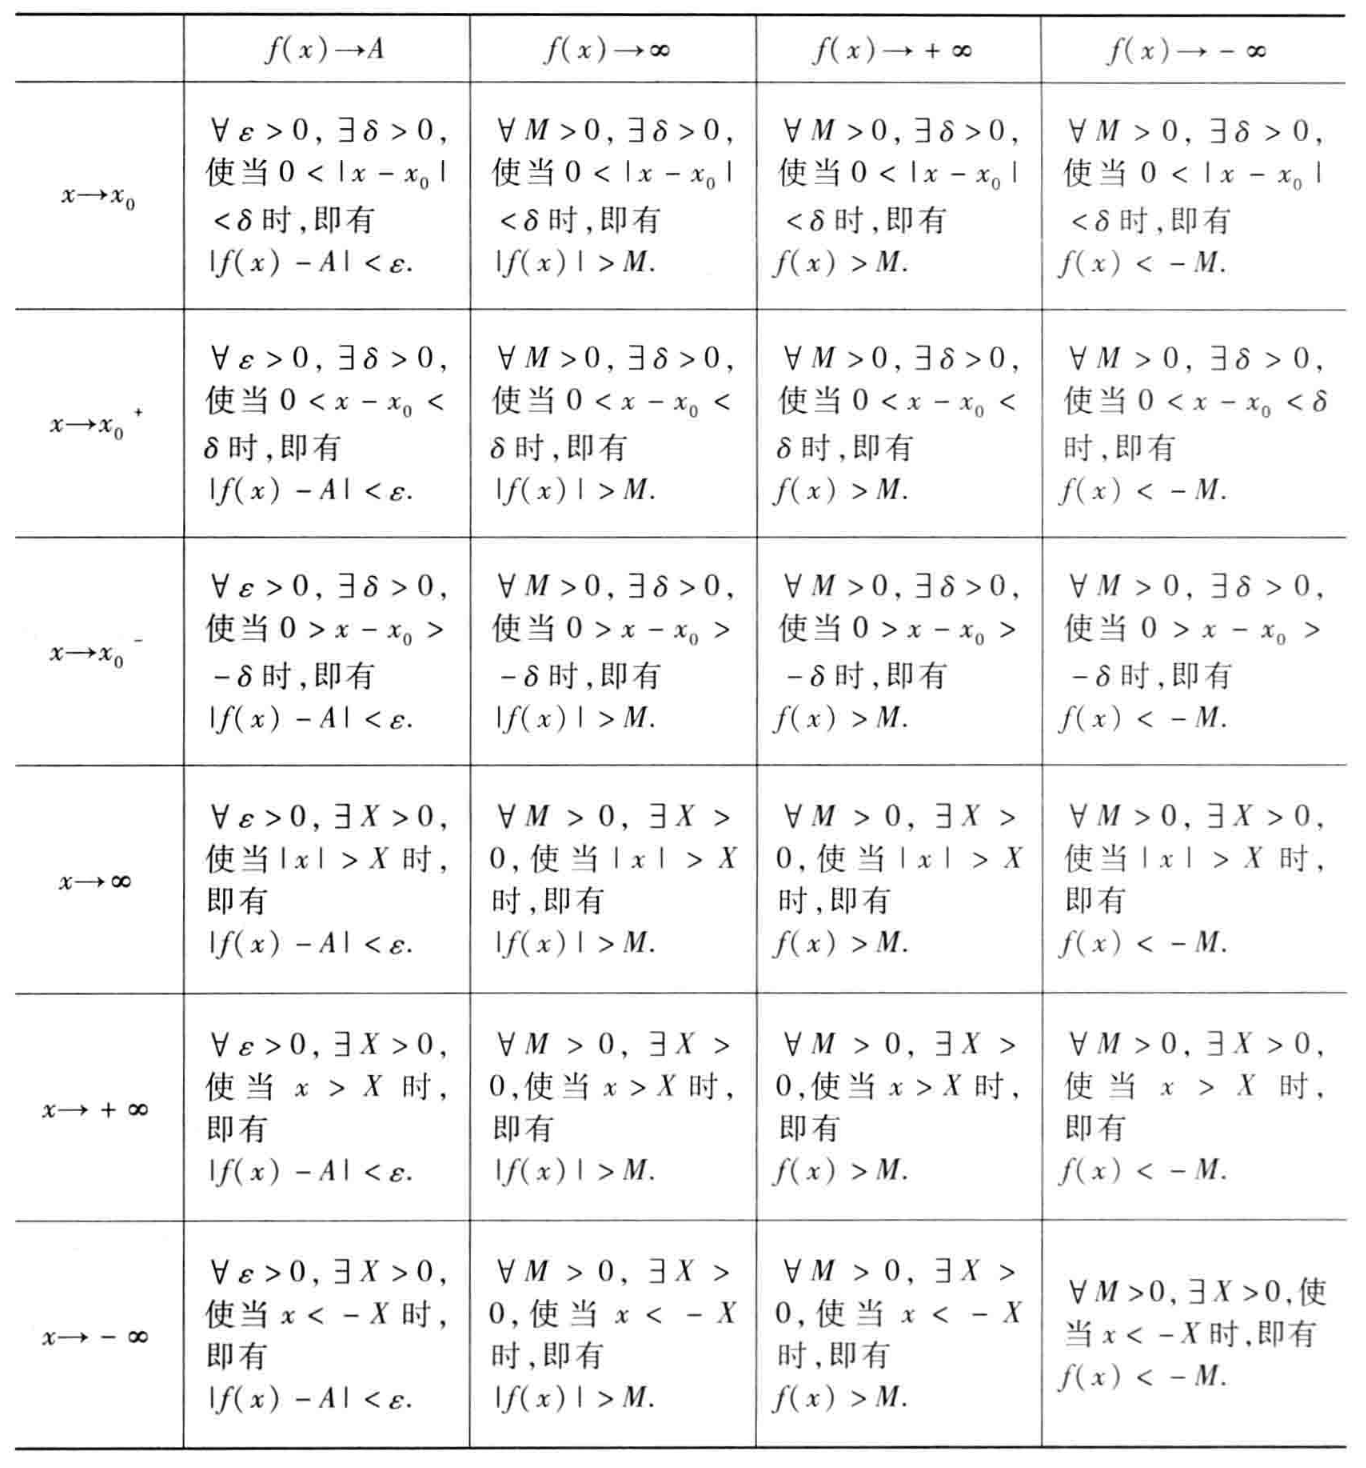
\includegraphics[width=\textwidth,height=0.8\textheight,keepaspectratio]{epsilon-delta.png}
	\end{figure}
\end{frame}

\begin{frame}
	\frametitle{证明题}

	\begin{block}{题目}
		\begin{itemize}
			\item $\lim\limits_{x \to 3}(3x-1)=8$,
			\item $\lim\limits_{x \to 2}(5x+2)=12$,
			\item $\lim\limits_{x \to -2} \displaystyle\frac{x^2-4}{x+2}=-4$,
			\item $\lim\limits_{x \to -\frac{1}{2}} \displaystyle\frac{1-4x^2}{2x+1}=2$.
		\end{itemize}
	\end{block}
\end{frame}

\begin{frame}{利用多项式计算的计算方法(注意分母为零的情况)}
	\begin{exampleblock}{定理}
		对于一个多项式函数 $P(x)$, 当 $x$ 趋向于某个实数 $a$ 时, $P(x)$ 的极限是 $P(a)$, 即
		\[
			\lim_{x \to a} P(x) = P(a)
		\]
	\end{exampleblock}
	\begin{block}{极限的四则运算}
		对于 $x_0,  A,  B,  k \in \mathbb{R}$,  如果有 $\lim _{\substack{x \rightarrow x_0 \\(x \rightarrow \pm\infty)}} f(x)=A$ 和 $ \lim _{\substack{x \rightarrow x_0 \\(x \rightarrow \pm\infty)}} g(x)=B$,   则有:

		\begin{enumerate}
			\item $\lim _{\substack{x \rightarrow x_0 \\(x \rightarrow \pm\infty)}}[f(x) \pm g(x)]=A \pm B$,  \\
			\item
			      $\lim _{\substack{x \rightarrow x_0 \\(x \rightarrow \pm\infty)}}[k f(x)]=k A$,  \\
			\item $\lim _{\substack{x \rightarrow x_0 \\(x \rightarrow\pm \infty)}}[f(x) \cdot g(x)]=A B$,  \\
			\item $\lim _{\substack{x \rightarrow x_0 \\(x \rightarrow\pm \infty)}} \displaystyle\frac{f(x)}{g(x)}=\frac{A}{B} \quad{\bf(B \neq 0)}$.
		\end{enumerate}
	\end{block}
\end{frame}


\begin{frame}
	\frametitle{计算题}

	\begin{block}{题目}
		\begin{columns}[onlytextwidth]
			\begin{column}{0.5\textwidth}
				\begin{enumerate}
					\item $\displaystyle\lim\limits_{h \to 0} \frac{(x+h)^2-x^2}{h}$,
					\item $\displaystyle\lim\limits_{x \to \infty} \frac{x^2-1}{2x^2-x-1}$,
					\item $\displaystyle\lim\limits_{x \to \infty}\left(1+\frac{1}{x}\right)\left(2-\frac{1}{x^2}\right)$,
				\end{enumerate}
			\end{column}
			\begin{column}{0.5\textwidth}
				\begin{enumerate}
					\setcounter{enumi}{3}
					\item $\displaystyle\lim\limits_{x \to 1}\left(\frac{1}{1-x}-\frac{3}{1-x^3}\right)$,
					\item $\displaystyle\lim _{x \rightarrow 2} \frac{x^3+2 x^2}{(x-2)^2}$,
					\item $\displaystyle\lim _{x \rightarrow \infty} \frac{x^2}{2 x+1}$.
				\end{enumerate}
			\end{column}
		\end{columns}
	\end{block}
	\pause
	\begin{exampleblock}{答案}
		\begin{columns}[onlytextwidth]
			\begin{column}{0.5\textwidth}
				\begin{enumerate}
					\item $2x$,
					      \pause
					\item $1/2$,
					      \pause
					\item $2$,
				\end{enumerate}
			\end{column}
			\begin{column}{0.5\textwidth}
				\begin{enumerate}
					\setcounter{enumi}{3}
					\pause
					\item $-1$,
					      \pause
					\item $+\infty$,
					      \pause
					\item $\infty$.
				\end{enumerate}
			\end{column}
		\end{columns}
	\end{exampleblock}

\end{frame}

\begin{frame}{利用重要极限$\displaystyle\lim_{x\to0}\frac{\sin x}{x}=1$ (注意分母为不零的情况)}
	\begin{block}{题目}
		\begin{columns}[onlytextwidth]
			\begin{column}{0.5\textwidth}
				\begin{enumerate}
					\item $\displaystyle\lim _{x \rightarrow 0} \frac{\sin \omega x}{x}$
					\item $\displaystyle\lim _{x \rightarrow 0} \frac{\tan 3 x}{x}$
					\item $\displaystyle\lim _{x \rightarrow 0} \frac{\sin 2 x}{\sin 5 x}$
				\end{enumerate}
			\end{column}
			\begin{column}{0.5\textwidth}
				\begin{enumerate}
					\setcounter{enumi}{3}
					\item $\displaystyle\lim _{x \rightarrow 0} x \cot x$
					\item $\displaystyle\lim _{x \rightarrow 0} \frac{1-\cos 2 x}{x \sin x}$
					\item $\displaystyle\lim _{n \rightarrow \infty} 2^n \sin \frac{x}{2^n}$
				\end{enumerate}
			\end{column}
		\end{columns}
	\end{block}
	\begin{exampleblock}{答案}
		\begin{columns}[onlytextwidth]
			\begin{column}{0.5\textwidth}
				\begin{enumerate}
					\item $\omega$,
					      \pause
					\item $3$,
					      \pause
					\item $\displaystyle\frac{2}{5}$,
				\end{enumerate}
			\end{column}
			\begin{column}{0.5\textwidth}
				\begin{enumerate}
					\setcounter{enumi}{3}
					\pause
					\item $1$,
					      \pause
					\item $2$,
					      \pause
					\item $x$.
				\end{enumerate}
			\end{column}
		\end{columns}
	\end{exampleblock}
\end{frame}

\begin{frame}{利用重要极限$\displaystyle\lim_{n\to0}(1+\frac{1}{n})^n=\mathrm{e}$ (注意变量变换)}
	\begin{block}{题目}
		\begin{columns}[onlytextwidth]
			\begin{column}{0.5\textwidth}
				\begin{enumerate}
					\item $\displaystyle\lim _{x \rightarrow 0}(1-x)^{\frac{1}{x}}$,
					\item $\displaystyle\lim _{x \rightarrow 0}(1+2 x)^{\frac{1}{x}}$,
				\end{enumerate}
			\end{column}
			\begin{column}{0.5\textwidth}
				\begin{enumerate}
					\setcounter{enumi}{2}
					\item $\displaystyle\lim _{x \rightarrow \infty}\left(\frac{1+x}{x}\right)^{2 x}$,
					\item $\displaystyle\lim _{x \rightarrow \infty}\left(1-\frac{1}{x}\right)^{k x}$.
				\end{enumerate}
			\end{column}
		\end{columns}
	\end{block}
	\begin{exampleblock}{答案}
		\begin{columns}[onlytextwidth]
			\begin{column}{0.5\textwidth}
				\begin{enumerate}
					\item $e^{-1}$,
					      \pause
					\item $e^2$,
				\end{enumerate}
			\end{column}
			\begin{column}{0.5\textwidth}
				\begin{enumerate}
					\setcounter{enumi}{2}
					\pause
					\item $e^2$
					      \pause
					\item $e^{-k}$.
				\end{enumerate}
			\end{column}
		\end{columns}
	\end{exampleblock}
\end{frame}

\begin{frame}
	\frametitle{等价无穷小的定义}
	\begin{block}{无穷小的比较和定义}
		对于函数$f(x)$和$g(x)$, 如果当$x$趋于某一点$a$时, $f(x)$的极限为$0$, $g(x)$的极限也为$0$, 如果有
		\[
			\lim_{x\to a}\frac{g(x)}{f(x)}=L.
		\]
		那么在 $L=0$ 时, 称 $g(x)$ 是 $f(x)$ 的高阶无穷小, 记作$g(x)= o(f(x))$; $L\neq0$ 时, 称 $g(x)$ 和 $f(x)$ 是同阶无穷小; 特别地, 在 $L=1$时, 则称 $g(x)$ 和 $f(x)$ 是等价无穷小, 记作 $g(x)\sim f(x)$.
	\end{block}
\end{frame}

\begin{frame}
	\frametitle{习题: 无穷小的判断 }
	\begin{block}{题目 $(\text{如果没有特别提及, 考虑 }\,\,x\to0)$}
		\begin{columns}[onlytextwidth]
			\begin{column}{0.5\textwidth}
				\begin{enumerate}
					\item $-2x-x^2$, $x^2-x^3$;
					\item $(1-\cos x)^2$, $\sin^2 x$;
					\item $1-x$, $1-x^3$, $\frac{1}{2}(1-x^2)$, $(x\to1)$;
					\item $\sqrt{1+x}-1, x$
				\end{enumerate}
			\end{column}
			\begin{column}{0.5\textwidth}
				\begin{enumerate}
					\setcounter{enumi}{4}
					\item $\displaystyle\sqrt[n]{1+x}-1$, $\displaystyle\frac{x}{n}$
					\item $\arctan x$, $x$;
					\item $\sec x-1$, $\displaystyle\frac{x^2}{2}$;
					\item $\tan x-\sin x$, $\sin^3 x$.
				\end{enumerate}
			\end{column}
		\end{columns}
	\end{block}
	\begin{exampleblock}{答案}
		\begin{columns}[onlytextwidth]
			\begin{column}{0.5\textwidth}
				\begin{enumerate}
					\item $x^2-x^3=o(-2x-x^2)$;
					      \pause
					\item $(1-\cos x)^2=o(\sin^2 x)$;
					      \pause
					\item $1-x \sim \frac{1}{2}(1-x^2)$, 与 $1-x^3$ 同阶;
					      \pause
					\item 同阶;
				\end{enumerate}
			\end{column}
			\begin{column}{0.5\textwidth}
				\begin{enumerate}
					\setcounter{enumi}{4}
					\pause
					\item $\displaystyle\sqrt[n]{1+x}-1\sim\displaystyle\frac{x}{n}$,
					      \pause
					\item $\arctan x\sim x$;
					      \pause
					\item $\sec x-1\sim\displaystyle\frac{x^2}{2}$;
					      \pause
					\item 同阶.
				\end{enumerate}
			\end{column}
		\end{columns}
	\end{exampleblock}
\end{frame}

\begin{frame}{连续函数性质相关的习题}
	\begin{exampleblock}{间断点分类: 名称}
		\begin{equation*}
			\text{间断点}\left\{
			\begin{array}{ll}
				\text{第一类间断点}\left\{
				\begin{array}{ll}
					\text{可去间断点} \\
					\text{跳跃间断点(跃点)}
				\end{array}
				\right. \\
				\text{第二类间断点}
			\end{array}
			\right.
		\end{equation*}
	\end{exampleblock}
	\pause
	\begin{block}{题目(判断函数的连续性和间断性)}
		\begin{columns}[onlytextwidth]
			\begin{column}{0.5\textwidth}
				\begin{enumerate}
					\item $f(x)= \begin{cases}x^2, & 0 \leqslant x \leqslant 1, \\ 2-x, & 1<x \leqslant 2;\end{cases}$
					\item $f(x)= \begin{cases}x, & -1 \leqslant x \leqslant 1, \\ 1, & x<-1 \text { 或 } x>1 ;\end{cases}$
				\end{enumerate}
			\end{column}
			\begin{column}{0.5\textwidth}
				\begin{enumerate}
					\setcounter{enumi}{2}
					\item $\displaystyle f(x)=\lim _{n \rightarrow-\infty} \frac{1-x^{2 n}}{1+x^{2 n}} x$;
					\item $y=\left\{\begin{array}{l}x-1,\quad x \leqslant 1, \\ 3-x,\quad x>1.\end{array}\right.$
				\end{enumerate}
			\end{column}
		\end{columns}
	\end{block}
\end{frame}

\begin{frame}{复合运算性质相关计算}
	\begin{block}{连续函数映射和求极限的可交换性}
		设函数$f(x)$在点$a$处连续, 且$\lim_{x\to a}g(x)=b$, 则有
		\[\lim_{x\to a}f(g(x))=f(\lim_{x\to a}g(x))=f(b)\]
		即连续函数映射和求极限可以交换顺序.
	\end{block}
	\pause
	\begin{block}{}
		\begin{columns}[onlytextwidth]
			\begin{column}{0.3\textwidth}
				\begin{enumerate}
					\item $\displaystyle \lim _{x \rightarrow \infty} e^{\frac{1}{x}}$, \pause\,\, $1$;\pause
					\item $\displaystyle \lim _{x \rightarrow 0} \ln \frac{\sin x}{x}$, \pause\,\, $0$;\pause
					\item $\displaystyle \lim _{x \rightarrow \infty}\left(1+\frac{1}{x}\right)^{\frac{x}{2}}$,\pause  \,\,$e^\frac{1}{2}$;\pause
					\item $\displaystyle \lim _{x \rightarrow 0}\left(1+3 \tan ^2 x\right)^{\cot x}$,\pause\,\,$e^3$;\pause
				\end{enumerate}
			\end{column}
			\begin{column}{0.55\textwidth}
				\begin{enumerate}
					\setcounter{enumi}{4}
					\item $\displaystyle \lim _{x \rightarrow \infty}\left(\frac{3+x}{6+x}\right)^{\frac{x-1}{2}}$,\,\,\pause $e^{-\frac{3}{2}}$;\pause
					\item $\displaystyle \lim _{x \rightarrow 0} \frac{\sqrt{1+\tan x}-\sqrt{1+\sin x}}{x \sqrt{1+\sin ^2 x}-x}$,\,\,\pause $\displaystyle\frac{1}{2}$;\pause
					\item $\displaystyle \lim _{x \rightarrow e} \frac{\ln x-1}{x-e}$,\,\,\pause $e^{-1}$;\pause
					\item $\displaystyle \lim _{x \rightarrow 0} \frac{e^{3 x}-e^{2 x}-e^x+1}{\sqrt[3]{(1-x)(1+x)}-1}$,\,\,\pause $-6$.
				\end{enumerate}
			\end{column}
		\end{columns}
	\end{block}
\end{frame}

\begin{frame}
	\begin{block}{介值定理}
		设 $y=f(x)$ 在 $[a, b]$ 上连续, $M$ 和 $m$ 为 $y=f(x)$ 在 $[a, b]$ 上的最大值和最小值, 则任给值 $c$ : $m<c<M$, 存在 $\xi \in(a, b)$, 使得 $f(\xi)=c$.
	\end{block}
	\pause
	\begin{block}{}
		设$f(x)=x-a \sin x-b$, 证明方程$f(x)=0$至少有一个正根, 并且它不超过$a+b$.
	\end{block}
	\pause
	\begin{block}{}
		证明任一最高次项指数为奇数的代数方程
		$$
			a_0 x^{2 n+1}+a_1 x^{2 n}+\cdots+a_{2 n} x+a_{2 n+1}=0,
		$$

		至少有一实根, 其中 $a_0, a_1, \cdots, a_{2 n+1}$ 均为常数, $n \in \mathbf{N}$.
	\end{block}
\end{frame}

% Thank you page
\beamertemplateshadingbackground{structure.fg!90}{structure.fg}
\begin{frame}[plain]
	\vfill
	\centering
	{
		\centering \Huge \color{white} Thank you for your attention!\\[10pt]Questions?\\
	}
	\vfill
\end{frame}
\end{document}


